% !TEX encoding = UTF-8
% !TEX program = pdflatex
% !TEX root = MEMOC.tex
% !TEX spellcheck = it-IT

%\chapter{Meta-euristiche}
%\section{Local Search}

\subsection{Soluzione di partenza}

Il modo più semplice di ottenere una soluzione di partenza è quello di generarne una casualmente. Oppure se il problema deriva da un caso reale può essere che ci sia già una soluzione attualmente utilizzata che può essere utilizzata come base di partenza.
Un'altra idea è quella di partire da una soluzione buona ottenuta con un'euristica veloce. Tanto non c'è una scelta migliore a livello teorico, c'è quindi un trade-off tra il tempo investito per trovare una buona soluzione di partenza o quello per la ricerca dell'ottimo.
Ovviamente c'è sempre il rischio di incastrarsi in un massimo locale.

Se si sceglie una soluzione di partenza generata casualmente è possibile ripetere la ricerca locale più volte in modo da trovare più soluzioni ottime locali, nella speranza che una di queste sia migliore delle altre o una soluzione ottima globale.

\subsection{Rappresentazione di una soluzione}

Il modo in cui viene rappresentata la soluzione è importante perché va ad influire sulla definizione del vicinato e alla forma dello spazio di ricerca.

Con rappresentazione della soluzione non si intende l'utilizzo di un vettore piuttosto di una lista, ma ad un livello più astratto.
Ad esempio per il problema dello zaino è possibile rappresentare la soluzione con un vettore binario, dove un 1 indica che l'elemento è stato messo nello zaino, oppure come una pila di oggetti che rappresentano i vari elementi.

In base alla codifica può anche essere necessaria una decodifica per ottenere un risultato comprensibile dalle persone.

\subsection{Definizione del vicinato}

Data una soluzione \textit{x}, le sue soluzioni vicine sono quelle che si ottengono applicando delle \textit{mosse} che modificano \textit{x}. Ad esempio l'aggiunta di un elemento nello zaino o la rimozione di un altro.

Tipicamente si tratta di piccole modifiche e quindi la \textbf{dimensione} del vicinato è piccola, per renderne la valutazione veloce. Tuttavia c'è un trade-off, perché al crescere del vicinato diminuisce la probabilità di convergere ad un ottimo locale, ma aumenta la complessità/tempo per la generazione/valutazione.

Bisogna quindi tenere conto anche della complessità dell'algoritmo di valutazione, perché deve essere eseguito su tutte le soluzioni presenti nel vicinato.

L'obiettivo è quindi quello di definire un \textbf{vicinato forte}, ovvero che ha delle buon probabilità di produrre delle soluzioni ottime locali, questo perché se si ha a disposizione un vicinato forte è più facile raggiungere una buona soluzione anche a partire da una soluzione pessima.

Un'altra proprietà desiderabile è quella della \textbf{connection}, ovvero che date due soluzioni feasible sia sempre possibile trovare una sequenza di mosse che permetta di passare da una soluzione all'altra. Se non c'è questa proprietà, la probabilità di ottenere una buona soluzione cala.

\subsubsection{Rappresentazione e l'influenza sul vicinato}

Per il problema dello zaino possiamo utilizzare 3 rappresentazioni:

\begin{itemize}
	\item Una lista con gli elementi inseriti nello zaino.
	\item Un vettore booleano con tanti valori quanti sono gli elementi totali. Un 1 indica che l'elemento è nello zaino.
	\item Uno stack con gli elementi.
\end{itemize}

Considerando come mosse l'aggiunta di un elemento e lo swap, non si ottengono dei vicinati connessi, perché può essere che per passare da un soluzione ad un'altra migliore sia necessari fare una mossa non ottima.

Ma c'è anche un problema pratico, implementare l'inserimento/swap in una lista o vettore è semplice, ma sullo stack (o lista ordinata), l'implementazione può essere più complessa e in alcuni casi può non essere possibile.

\subsection{Funzione di valutazione}

Questa funzione viene utilizzata per definire la bontà di uno stato. 
Tipicamente viene utilizzata la funzione obiettivo, ma è possibile aggiungere delle feature extra come una somma di pesi, o delle penalità per dei vincoli non rispettati.
Modificando così la funzione di valutazione si riesce a far sembrare ``più buone'' delle soluzioni che in realtà sono peggiori di quella attuale, in modo da avere un vicinato connesso.

Ad esempio per il problema dello zaino si può considerare la funzione

$$
\overline{f}(x) = \alpha \sum_{i \in X} p_i - \beta\max\{0, \big(\sum_{i\in X} w_i\big)-W\}
$$

\noindent dove il secondo termine prende in considerazione lo spazio libero rimasto, così una soluzione che rimuove un elemento dallo zaino può essere vista come una soluzione migliore.

\subsection{Strategie di esplorazione}

Quando ci si sposta in una soluzione vicina, si cerca di migliorare il valore della funzione di valutazione.
L'idea greedy è quella di spostarsi sul vicino migliore (\textbf{steepest descent}), ma questo richiede di valutare tutto il vicinato.

Un'altra idea è quella di passare alla prima soluzione migliore (\textbf{first improvement}), ovvero man mano che si espande il vicinato, si effettua anche la valutazione e ci si sposta alla prima soluzione migliore che si trova. Così facendo però l'ordine in cui vengono generate le soluzioni vicine è influente sulla scelta della soluzione migliore.

Si può inoltre scegliere una soluzione a caso tra le $k$ migliori presenti nel vicinato, oppure si può tenere in memoria la seconda scelta in modo da avere un punto di partenza per una successiva ricerca.

\subsection{Esempio di Local Search su TSP}

TSP è un problema NP-Hard e già a partire da 100 nodi, CPLEX fa fatica a trovare una soluzione ottima con l'approccio esatto.

Come notazione del problema abbiamo un grafo $G = (V,A)$ completo e indiretto, $|V| = n$ e i costi di cammino sono indicati con $c_{i,j} = c_{j,i}$.

Dobbiamo quindi definire i componenti della ricerca locale.

\subsubsection{Soluzione iniziale}

Il modo più semplice per trovare una soluzione di partenza è prendere i nodi in modo causale.

\paragraph{Nearest Neighbour} Tuttavia si può fare meglio utilizzando un euristica greedy: viene scelto un nodo $i_0$ di partenza e ad ogni passo viene aggiunto il nodo $j$ tale che 
$$
j = \arg\min_{j\in V \setminus Cycle }
$$

\noindent fino a che non vengono aggiunti tutti i nodi.
L'euristica richiede un $O(n^2)$ e di per se non fornisce dei buoni risultati, ma è un buon punto di partenza per la ricerca locale.
Alcune varianti di questa euristica possono essere quelle di provare da vari nodi di partenza oppure di introdurre una scelta random tra gli archi di costo più basso.

\paragraph{Nearest/Farthest Insertion} 

In alternativa si può partire da un ciclo $C$ contenente i nodi $i$ e $j$ che sono i più vicini, ottenendo un costo $cost = c_{i,j} + c_{j,i}$. 

Il ciclo viene poi esteso andando ad aggiungere il nodo $r$ tale che

$$
r = \arg\min_{k \in V\setminus C} \{c_{k,j} : j \in C\}
$$

\noindent Il nodo $r$ viene poi aggiunto al ciclo tra i nodi $i$ e $j$, rendendo $cost = c_{i,r} + c_{r,j} - c_{i,j}$. 
Al passo successivo la procedura viene ripetuta selezionando all'interno del ciclo i due nodi che sono più vicini, il tutto finché non vengono inseriti tutti i nodi.

Esiste anche la variante Farthest che funziona in modo analogo ma con seleziona i nodi più lontani

La complessità dell'euristica è $O(n^3)$ e può essere sempre estesa con la randomizzazione.

\paragraph{Best Insertion}

Si parte costruendo un ciclo tra i due nodi più vicini e vengono via via aggiunti dei nodi tra i due nodi che sono più vicini.

$$
r = \arg\min_{i \in V\setminus C}\{c_{i,r} +c_{r,j} - c_{i,j}: i,j \text{ consecutivi } \in C\}
$$

\noindent Anche questa euristica ha complessità $O(n^3)$ e può essere randomizzata.

\subsubsection{Rappresentazione della soluzione}

Ci sono vari modi per rappresentare una soluzione:

\begin{itemize}
	\item \textbf{arc representation}: la soluzione è determinata dagli archi presenti nel percorso di costo minimo. Viene rappresentata con una matrice binaria di dimensione $n\times n$, contente un 1 negli archi che vengono attraversati.
	\item \textbf{adjancey representation}: i nodi vengono nominati da $1$ a $n$. Viene poi creato un vettore $v$ di lunghezza $n$, tale che l'elemento $v[i]$ rappresenta il nodo che viene visitato nel percorso dopo il nodo $i$.
	\item \textbf{path representation}: i nodi vengono memorizzati come una sequenza ordinata. Così facendo ogni soluzione è una permutazione dei nodi del grafo.
\end{itemize}

\noindent Come rappresentazione della soluzione utilizziamo la path representation perché è la più naturale e rappresenta sempre una soluzione ammissibile (anche adjancey gode di questa proprietà).

\subsubsection{Generazione del vicinato}

Per generare il vicinato utilizziamo \textbf{k-opt}, ovvero un algoritmo che rimuove $k$ archi dal ciclo della soluzione e ne aggiunge altri $k$ in modo che ci sia sempre un ciclo. Ovviamente non ha senso rimuovere archi che sono consecutivi tra loro.

\begin{figure}[htbp]
	\centering
	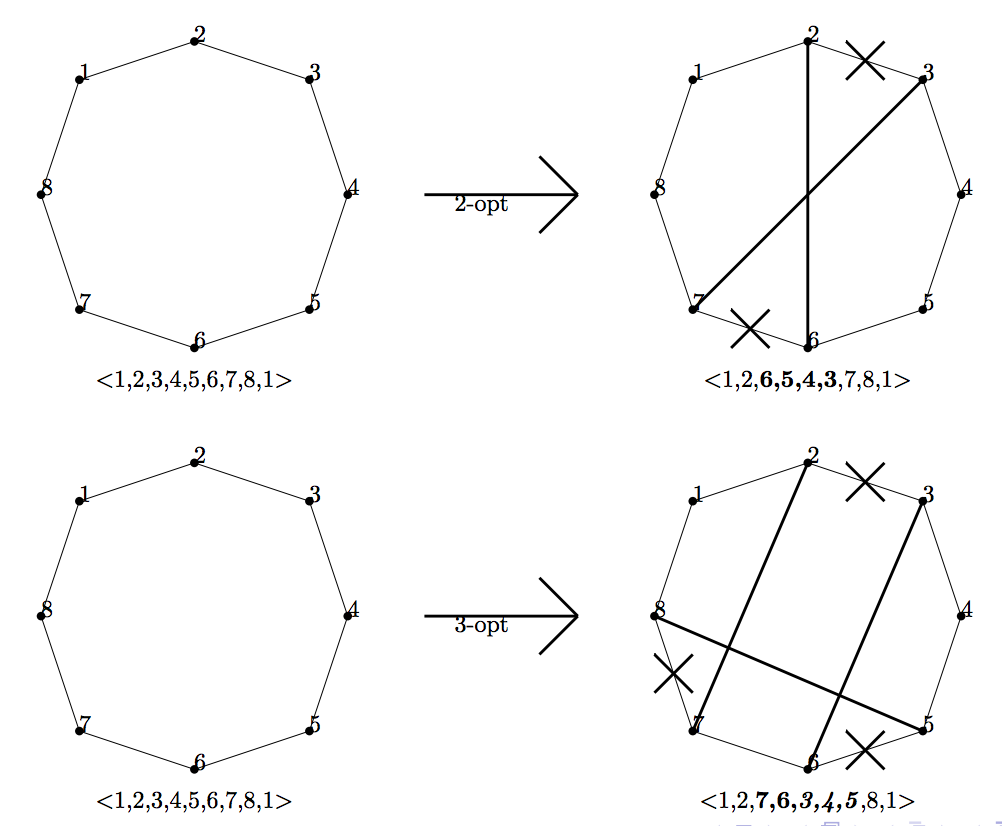
\includegraphics[width=0.7\textwidth]{images/l7-fig-1.png}
\end{figure}

\noindent Con 2-opt abbiamo una complessità $O(n^2)$ mentre nel caso generico si ha $O(n^k)$.

Fare una mossa con 2-opt equivale a effettuare una rotazione di una parte della sequenza di visita, ad esempio:

$$
\langle 1,2,3,4,5,6,7,8,1 \rangle \to\langle 1,2,6,5,4,2,7,8,1 \rangle 
$$

\noindent Questo può essere sfruttato per calcolare in modo incrementale il costo della nuova soluzione.

Assumendo che siano stati invertiti i nodi $i$ e $j$ con 2-opt, si ha che il nuovo costo può essere calcolato con 

$$
C_{new} = C_{old} - c_{i-1, i} - c_{j, j+1} + c_{i-1,j} + c_{i, j+1}
$$

\noindent questo risultato vale anche per $k$-opt, basta tenere in considerazione i costi che vengono tolti e aggiungere quelli nuovi. Il tutto funziona perché i costi sono simmetrici ($c_{i,j} = c_{j,i}$) e quindi anche se cambia il verso con il quale si attraversano gli archi, il costo non cambia.

Per quanto riguarda i valori di $k$, si è visto che già con 2 si ottengono dei buoni risultati, con 3 si ottengono dei buoni miglioramenti e con 4 i risultati migliorano, ma non abbastanza da giustificare l'aumento della complessità.

\subsubsection{Funzione di valutazione}

Non ci sono motivi per adottare una funzione diversa da quella obiettivo. Non ha senso andare ad introdurre delle penalità.

\subsubsection{Strategia di ricerca}

La ricerca può essere fatta sia con Steepest Descent che con First Improvement.


